\subsection{Lift and bucket for debris}

\subsubsection{Lift}
The lift consists of two beams. One beam is stationar and it is fixed vertically on the back part of the robot. The second beam turns by DC motor that mounted at the top of stationar beam. The length of beams must allow to score debris to the high goal from the middle zone and to middle goal from low zone.	\newline
For estimating optimal length of beams it was made drawing in GeoGebra.
\begin{figure}[H]
	\begin{minipage}[h]{1\linewidth}
		\center{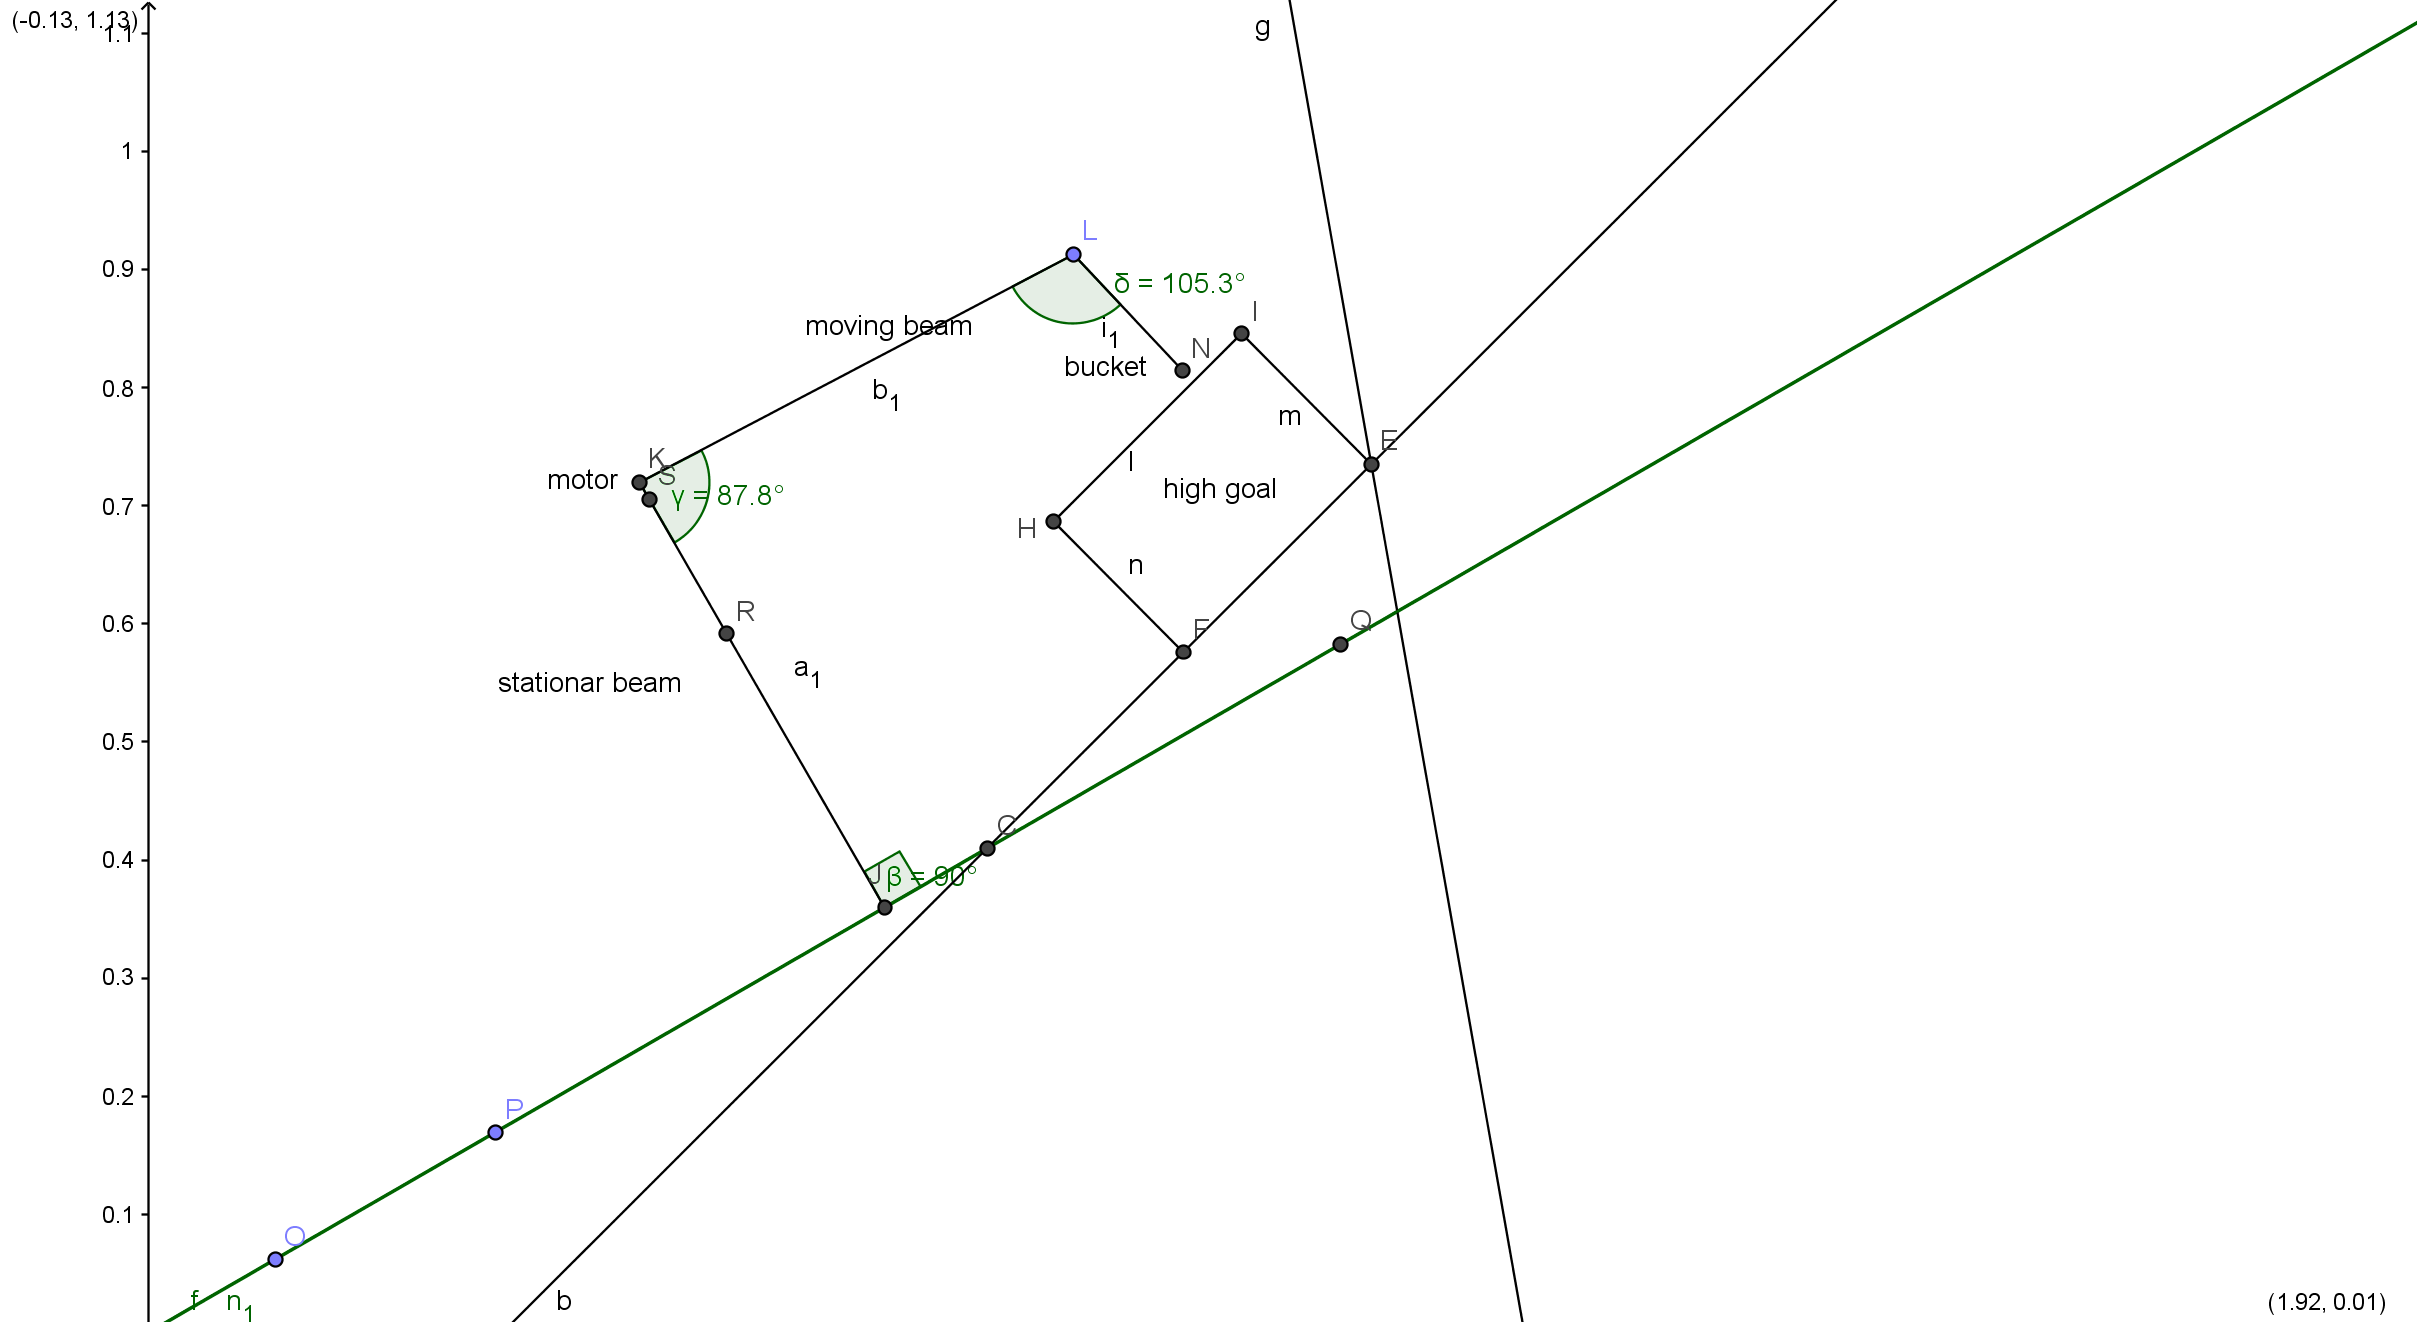
\includegraphics[scale=0.7]{3Engineering/6Specifications_for_modules/Lift+bucket/images/02}}
		\caption{Drawing of the lift}
	\end{minipage}
\end{figure}

\subsubsection{Bucket} 
The bucket's size allow to fit 3 cubes and 2 balls. So we can collect 5 cubes (because size of cube is smaller than size of ball) or 3-4 balls. It is enough for us because we want to concentrate on collecting cubes. 	\newline
For estimating optimal size and form it was made drawing in GeoGebra. During designing model of the bucket for all sizes were made dimention tolerances 2cm.
\begin{figure}[H]
	\begin{minipage}[h]{1\linewidth}
		\center{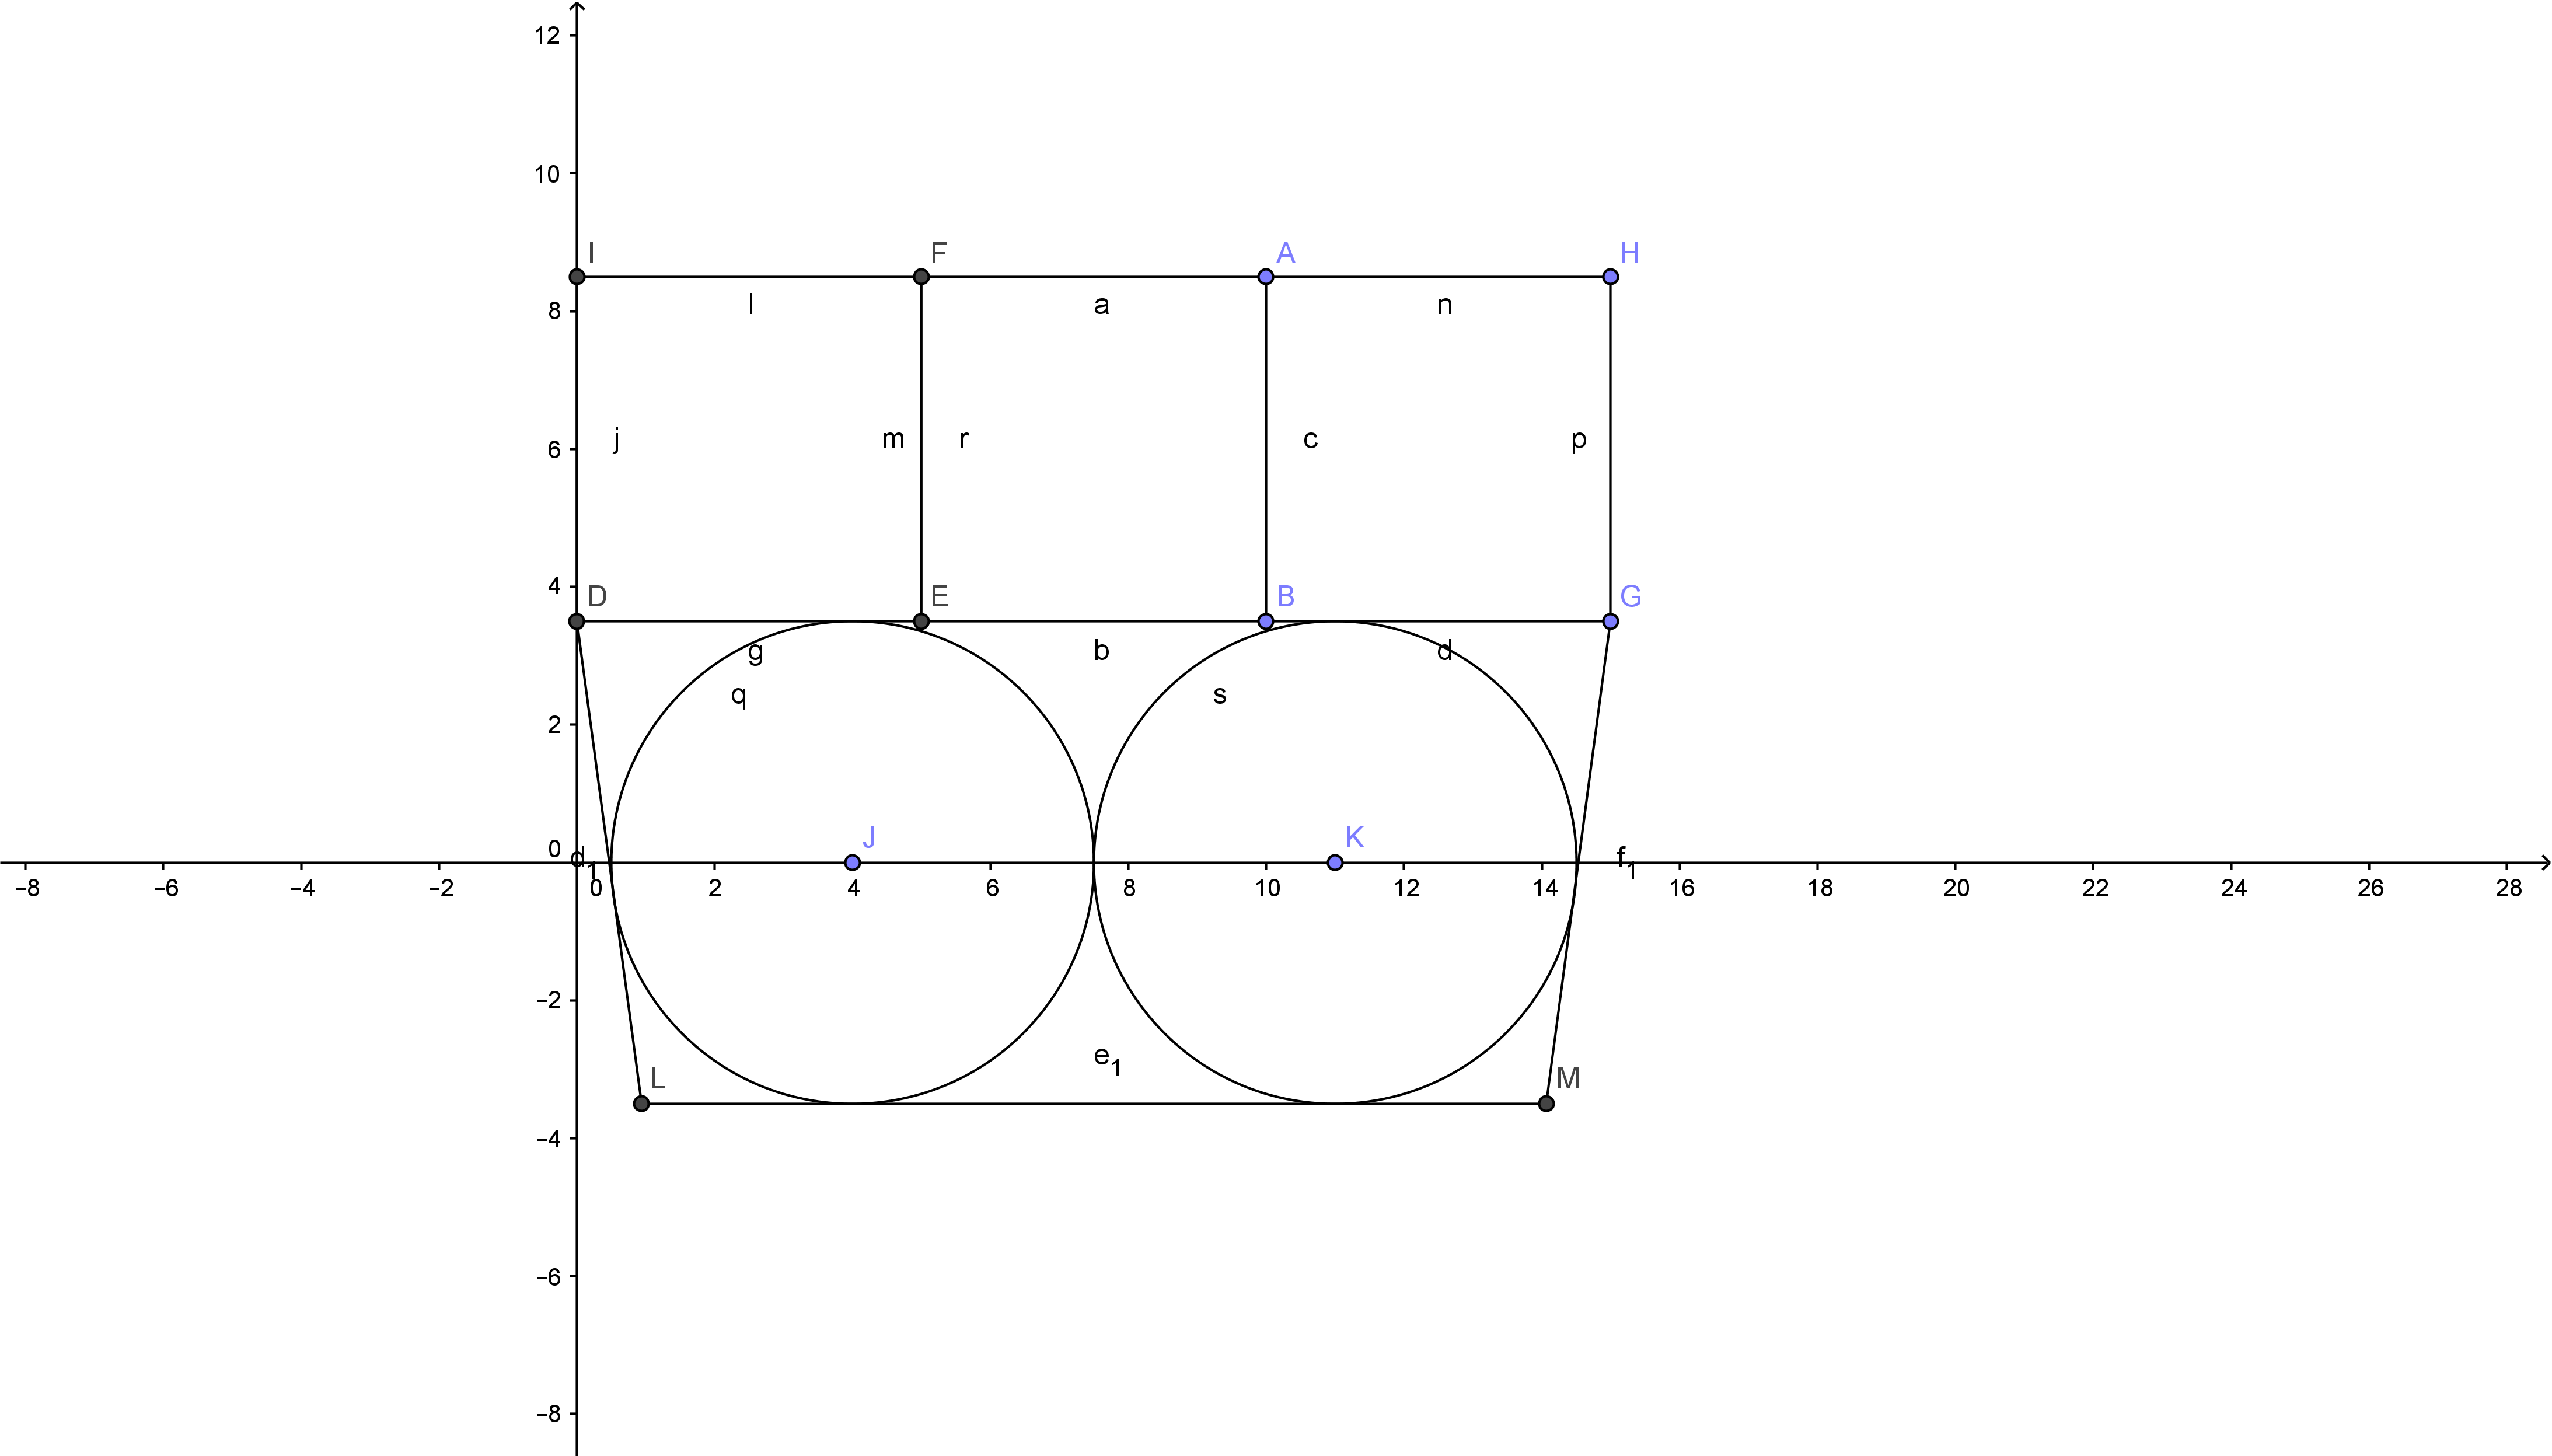
\includegraphics[scale=0.5]{3Engineering/6Specifications_for_modules/Lift+bucket/images/01}}
		\caption{Drawing of the bucket}
	\end{minipage}
\end{figure} 
But after that it was decided to change size of the bucket. The width entrance hole and width of the scoring box should be the same. It ensure maximal accuracy of scoring debris. It was decided to make bucket that can fit 5 cubes or 3 balls.
\begin{figure}[H]
	\begin{minipage}[h]{1\linewidth}
		\center{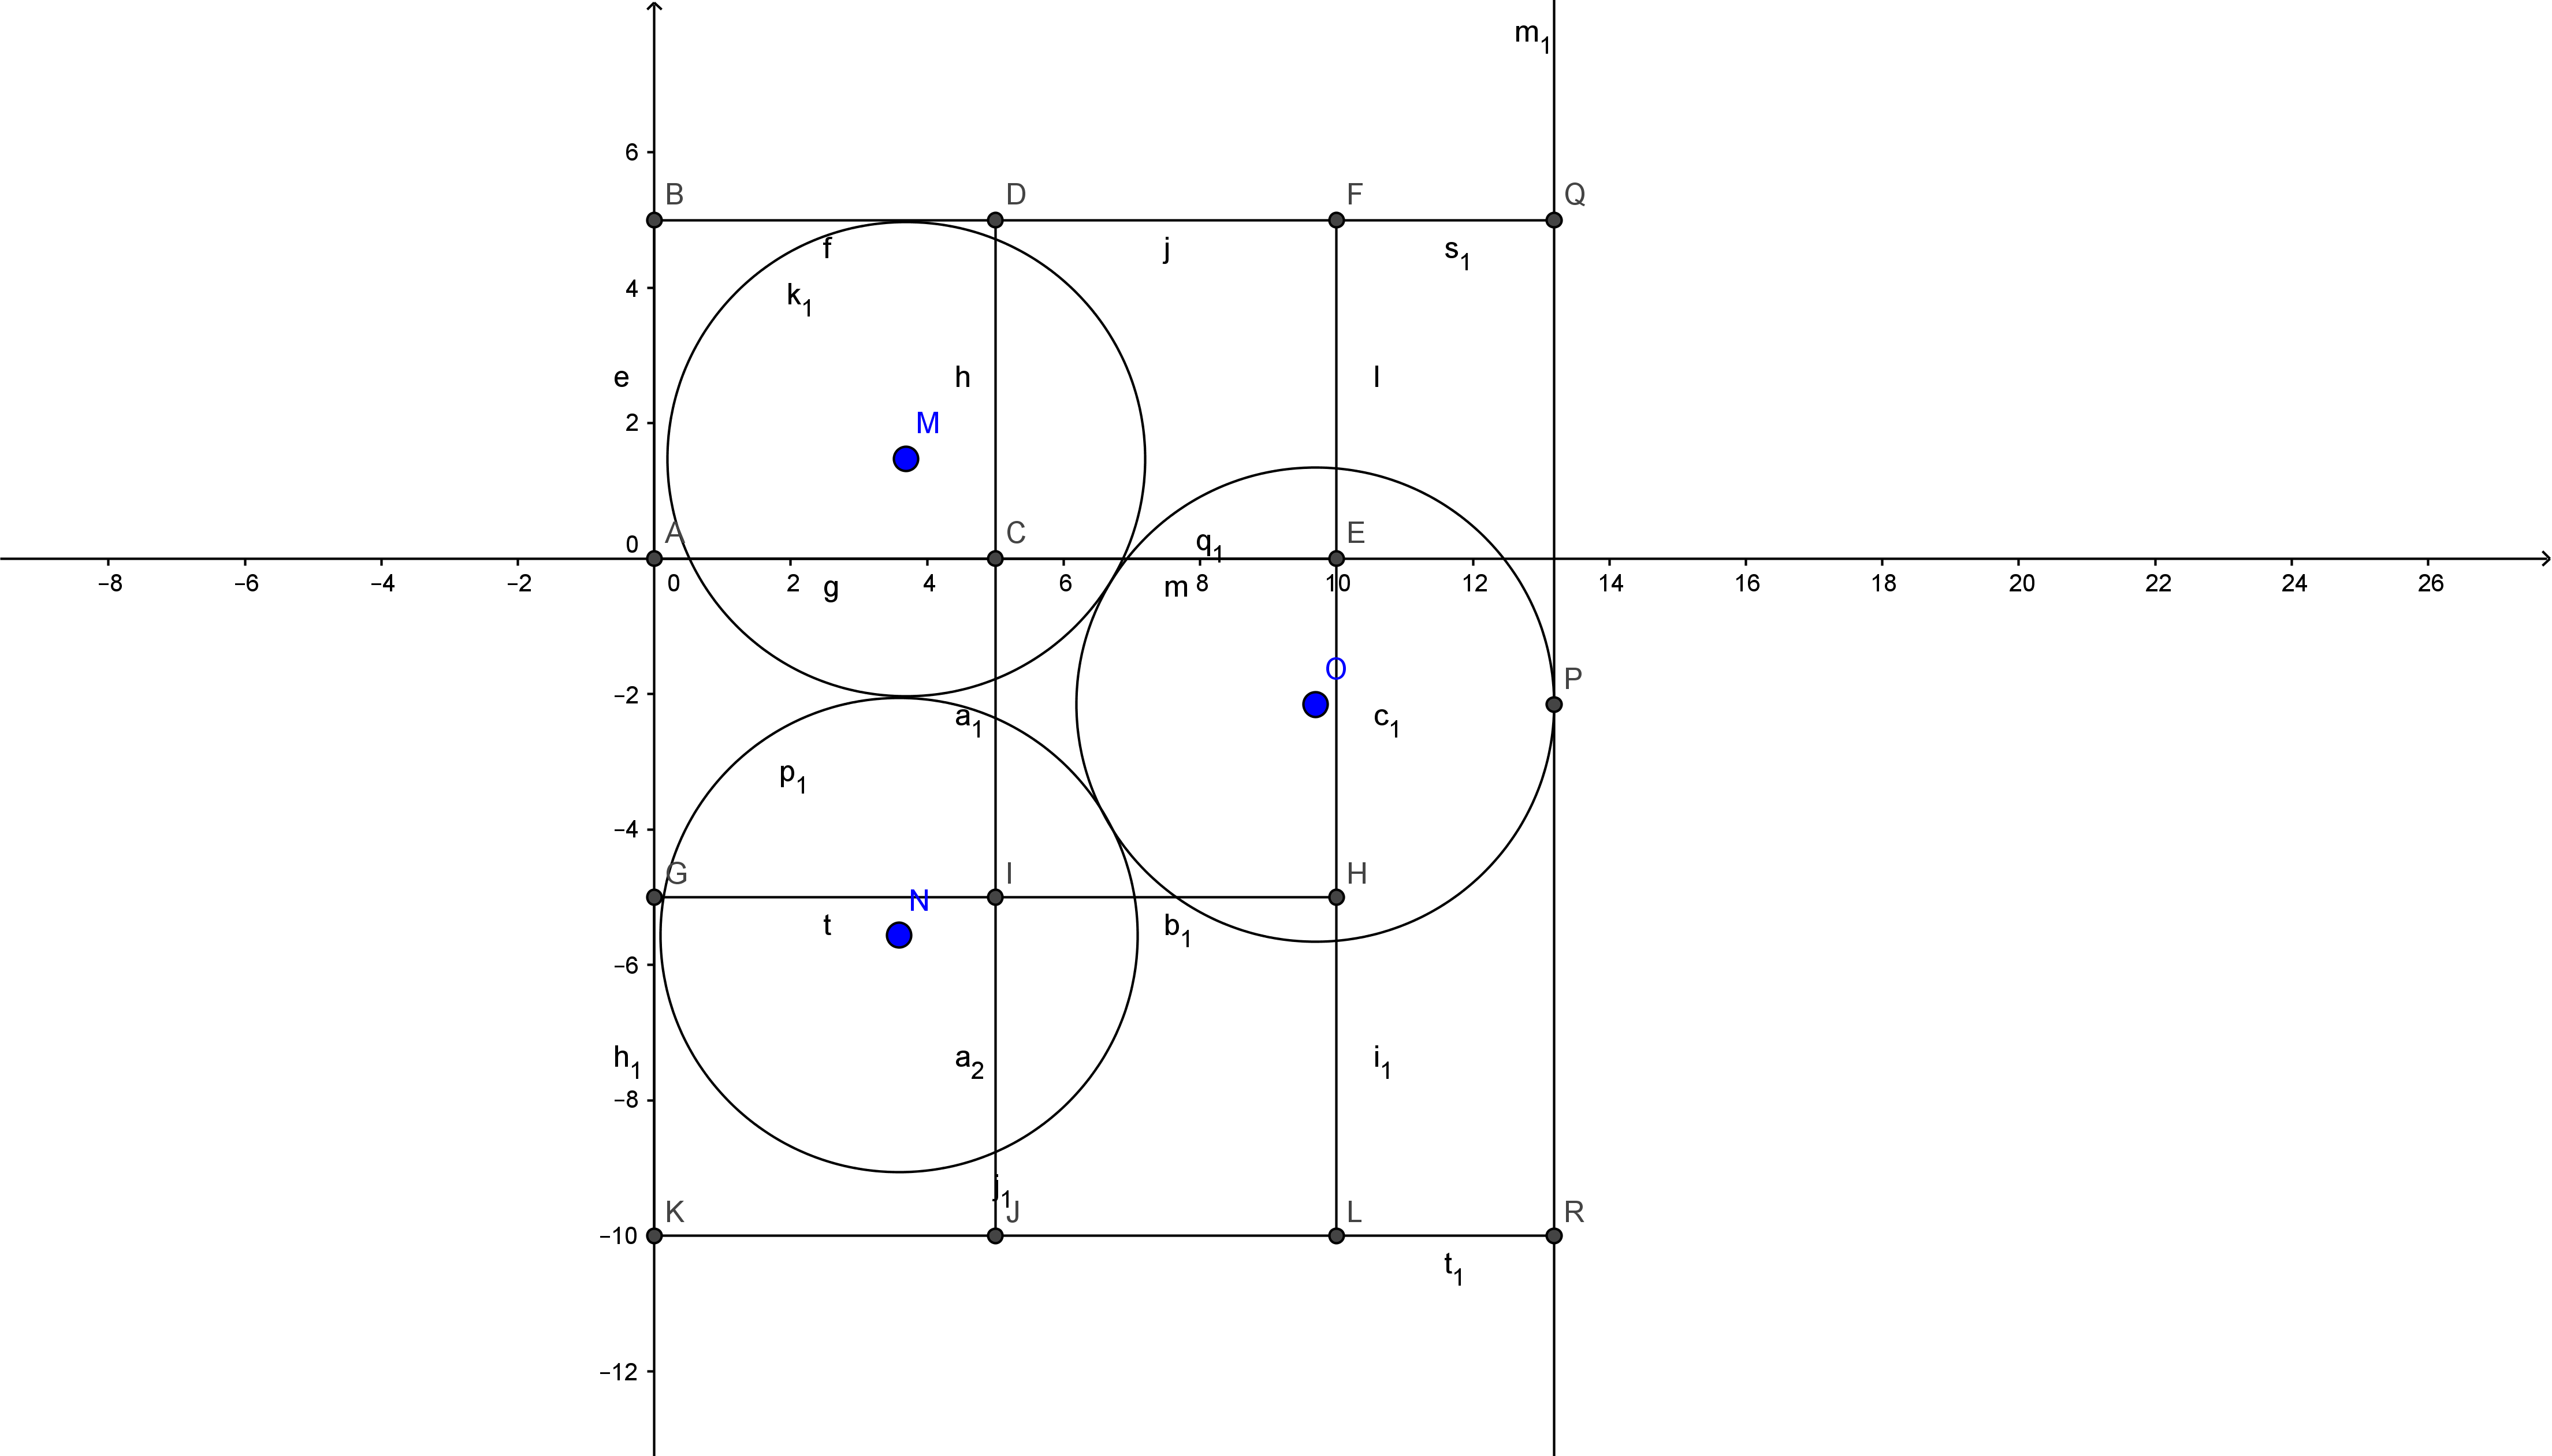
\includegraphics[scale=0.5]{3Engineering/6Specifications_for_modules/Lift+bucket/images/03}}
		\caption{Changed bucket}
	\end{minipage}
\end{figure}


For building bucket it was decided use plastic PET 0.5mm. It is easy to cut it, it light, cheap and clear that allow us to see how much elements are incide the bucket.\newline  

The bucket mounts to beam that turns by the servo which fixed on the lift. It need because else we have to make detail that fix bucket to the elevator on the defined angle. It require high accuracy. So it will be difficult to make this detail. In addition the mount with servo extend operational window of the lift. \newline

The bucket equped by the cover that turn by the servo and close entrance hole of the bucket. It prevent to falling debris out it during turning of the moving beam of lift. Also it can to prevent balls get into the bucket when we collect only cubes. When it closed not fully (so that distance between bottom edge of cover and floor is about 6cm) the cube can get into the bucket but the ball is not. When we open cover the balls can get to the bucket.\newline
The cover fix on 14cm beam that turn by the servo. It was decided use so long beam as the most optimal variant when cover move vertically because otherwise it can to prevent rotating gripper for debris. When it turn around the circle with big radius trajectory of cover's moving is close to vertical. \newline
Also they were calculated moments of force that acts to servos (for servo that turn bucket and for servo that move cover).



\fillpage
